
\documentclass{stat572Style}
\usepackage{natbib}
\usepackage{amssymb}
\usepackage{graphicx}
\usepackage{amsmath}
%%\setlength{\oddsidemargin}{0.25in}
%%\setlength{\textwidth}{6in}
%%\setlength{\topmargin}{0.5in}
%%\setlength{\textheight}{9in}

\renewcommand{\baselinestretch}{1.5} 

\bibliographystyle{plainnat}

\begin{document}
%%\maketitle

\begin{center}
  {\LARGE A Review of Lagrangian Time Series Models for Ocean Surface Drifter Trajectories (Sykulski et al. (2016))}\\\ \\
  {Hannah Director \\ 
    Department of Statistics, University of Washington Seattle, WA, 98195, USA
  }
\end{center}



%\begin{abstract}
%  Put your project summary here.
%\end{abstract}

\section{Introduction}
\indent ``Lagrangian Time Series Models for Ocean Surface Drifter Trajectories," by Adam M. Sykulski, Sofia C. Olhede, Jonathan M. Lilly, and Eric Danioux presents a multi-component spectral model for analysis of data transmitted by ocean surface drifters. Drifters are free-floating  instruments that transmit their location at regular time intervals,  creating a \textbf{\it{Langrangian time series}}, or a sequence of spatial locations over time. Oceanographers use these time series to increase understanding of  ocean circulation patterns. Published in January 2016 in the \textbf{\it{Journal of the Royal Statistical Society Series C}}, this paper develops a model that can isolate a scientific quantity of interest,  and, in so doing, introduces several new statistical techniques.\\
\indent The motion of parcels of water moving over changing latitudes is known to have a rotational component. Because the Earth has  different diameter at different latitudes, the speed of objects moving with Earth's rotation varies across latitudes.  This induces a phenomena known as the Coriolis Effect, whereby very fast moving objects or objects being observed over long periods, such as drifters, end up moving at speeds that are different than the Earth beneath them as they change latitude. Viewed from a stationary reference frame, this creates circular motions, or inertial oscillations. These motions have known frequencies, referred to as inertial frequencies. Oceanographers  are interested in detecting deviations from these frequencies, as they are thought to indicate eddies, or persistent circular wave patterns \citep{Kunze1985}. However, the ocean has a constant turbulent background flow which makes identifying eddies in real data difficult \citep{ Elipot2010}. The methods in this paper overcome this challenge and successfully find shifts in the inertial frequency with a spectral time series model. \\
\indent In achieving this result, several statistical advances are made.  The authors introduce an additive spectral domain model that has components corresponding to both the turbulent background and the inertial oscillations. For the turbulent background model, the Mat\'{e}rn covariance commonly used in spatial statistics \citep{Gneiting2012} is extended to the time-series context. This allows for a more flexible model for background behavior than previously obtained.  Inertial oscillations are modeled with a complex Ornstein-Uhlenbeck (OU) \citep{Arato1962, Jeffreys1968}, which provides a stochastic equivalent to an accepted set of coupled differential equations describing inertial oscillations. Further statistical innovation is employed in fitting the model with a variation on standard Whittle likelihood to reduce bias and in allowing for non-stationarity through time-varying parameter estimates. \\
\indent The remainder of this review proceeds as follows. After a succint review of spectral analysis, Section 2 discusses the model for the drifters and the methods used to fit it. Section 3 presents the paper's results including analysis of a long time series with time-varying parameters and an application from a simulated model. The paper concludes with a discussion of the value and limitations of the approach taken by \citet{Sykulski2016}. 
\section{Methods}
			

	\subsection{Spectral Analysis}
	\indent We briefly review spectral analysis as these methods are central to understanding \citet{Sykulski2016}.  More thorough coverage of this material can be found in  \citep{Percival1993}, for example. From a statistical perspective, a time series, $x(t)$ can be understood as a realization of a stochastic process over time, where  $t = \{1,2,...,n\}$ are the observed time points.  Time series are often modeled as the sums of periodic functions, which, using Euler's formula, can be represented compactly as Fourier series. Moreover, data in the time domain can easily be related to data in the frequency domain and vice versa using the Fourier or inverse Fourier transformations 	\begin{align}
x(t) \overset{ms}{=} \int_{-\infty}^{\infty} f_{x}(\omega)e^{i\omega t}d\omega && f_{x}(\omega) = \int_{-\infty}^{\infty} x(t) e^{-i \omega t }dt.
\end{align}
\citep{Percival1993}. To understand the distribution of frequencies, the \textbf{\it{power spectral density}},


\begin{equation}
S_{x}(\omega) = \underset{T \rightarrow \infty}{\lim} \mathbb{E} \left(\frac{1}{2T} \left| \int_{-T}^{T} x(t) e^{-i \omega t}dt \right|^{2} \right),
\end{equation}
is often employed. This quantity represents the variance (or power) associated with each frequency \citep{Percival1993}. Power spectral densities are useful for statistical modeling, since they can be related to the autocovariance sequence of a time series using  Fourier transformation.  Defining the autocovariance as $s_{x}(\tau) = \mathbb{E}[x(t) x(t - \tau)] $ where $\tau$ is the time lag, we have

\begin{align*}
S_{x}(\omega) = \int_{-\infty}^{\infty}s_{x}(\tau) e^{-\omega t}dt  \Longleftrightarrow s_{x}(\tau) = \frac{1}{2\pi} \int_{-\infty}^{\infty}S_{x}(\omega) e^{i \omega t} d\omega 
\end{align*}

\noindent \citep{Sykulski2013}. For an observed time series, the power spectral density is often estimated with the periodogram, $\hat{S}_{x}(\omega) = |J_{x}(\omega)|^{2}$ where 
\begin{equation}
J_{x}(\omega) = \sqrt{\frac{t}{N}} \sum_{t=1}^{N} x(t) e^{-i \omega t}
\end{equation}
\citep{Sykulski2013}. Although intuitively appealing, this estimator has known problems that stem from the sampling of a periodic function at discrete intervals. In particular,  high frequencies can  capture periodic behavior of other lower frequencies if that happen to align in period. Additionally, frequencies above the highest observable frequency cannot be captured, and, are instead, recorded as other frequencies in the spectrum.  These effects, referred to as $\textbf{\it{aliasing}}$ and $\textbf{\it{leakage}}$ respectively,  are typically reduced by $\textbf{\it{tapering}}$. This method uses  a window of frequencies for estimation rather than a single value. However, depending on how tapering is used, it can introduce its own  biases in estimation.  


\subsection{Model}
 To model the drifter's motion over time, the eastward and northward components of the drifter's velocity, denoted $u(t)$ and $v(t)$ respectively, are converted to a complex-valued velocity, $z(t) = u(t) + iv(t)$. Stochastic models are then developed for both components of the the drifter's behavior, inertial oscillations and movement due to the ocean's turbulent background,  in the spectral domain. Finally, the two components of the model are added together, creating a six-parameter model, which is fit via maximizing a blurred Whittle likelihood, a relatively new approximation to the true spectral likelihood that balances computational efficiency with minimizing bias \citep{Sykulski2013}. 
 
\subsubsection{Inertial oscillations}
We discuss modeling just the inertial oscillations first. In a deterministic setting, inertial oscillations are often modeled with the following set of coupled differential equations \citep{Pollard1970}
\begin{align}
\frac{\partial u }{\partial t}  + f_{0} \nu &= F - cu \\ \nonumber
\frac{\partial v}{\partial t} - f_{0}u &= G - cv
\end{align}
where $u$ and $v$ again represent eastward and northward velocities, $f_{0}$ represents the inertial frequency in radians per unit time, and $F$ and $G$ are forces related to the wind. Suppressing the dependence on $t$ and using the complex representation of the velocity, these relationships can be equivalently expressed as follows
\begin{align*}
\label{eq:diffEqDeriv}
\frac{dz}{dt} &= \frac{\partial u}{dt} + i\frac{\partial v(t)}{dt}\\
dz &= (F - c u- f_{0}v)dt + (iG - icv + if_{0}u)dt\\
&= fo(-v + iu)dt - c(u + iv)dt + (F + iG)dt\\
&= if_{0}(u + iv) - c(u + iv) + (F + iG)\\
&= (if_{0} - c)z dt + (F + iG)dt. 
\end{align*}
By further replacing the wind forcing term, $(F + iG)dt$, with complex-valued Brownian increments, \citet{Sykulski2016} obtain the stochastic model 
\begin{equation}
\label{eq:ouEq}
dz(t) = (i f_{0} -c) z(t) dt + A d Q(t), 
\end{equation}
which defines equivalent behavior to the accepted deterministic formulation. Equation ~\ref{eq:ouEq}  is known as the complex-valued Ornstein-Uhlenbeck (OU) stochastic differential equation. It developed from brownian motion to OU to complex OU, mean-reversion, dampening and is a valid in this context by  blah (look up and cite the Mandelrot and Van Ness justification) giving the This model is always Markovian. The OU model is stationary assuming the initial conditions of the stochastic differential equation are set as $z(t_{0}) \sim N(0, A^{2}/2|c|)$, and, if not, will revert to the stationary model quickly as the influence of the initial conditions decays exponentially (WHY? look this up). 

\citet{Sykulski2016} further let $f_{0}$ be a free parameter, denoted $\omega_{0}$, to be estimated by data. In so doing, they enable  identification and estimation of the shifts in the angular frequency due to eddies. If the estimated angular frequency differs from the inertial frequency, the angular frequency of the eddy can be calculated as $\omega_{eddy} = f_{0} - \omega_{0}$, since $\omega_{0}$ is a sum of the inertial and eddy frequencies.

Letting $z^{*}(t)$ represent the complex conjugate of z(t) and using the previously-specified initial conditions, the complex OU process has the following  autocovariance  and power spectral density
\begin{align}
\label{eq:ouAC}
s^{(0)}(\tau) &= \mathbb{E}\{z(t)z^{*}(t + \tau) \} = \frac{A^{2}}{2c} \exp(i \omega_{0}\tau) \exp(-c|\tau|)\\
\label{eq:ouPSD}
S^{(0)}(\omega) &= \int_{-\infty}^{\infty} s^{(0)}(\tau) \exp (-i \omega \tau) d \tau = \frac{A^{2}}{(\omega - \omega_{0}) + c^{2}}
\end{align}
where $\tau$ is a time lag and the $(o)$ subscripts denotes that these equations are for the OU component of the model.  In addition to the inertial frequency, $\omega_{0}$, the parameter, $A > 0$ that defines the variability, and the parameter, $c >0$ which controls the dampening,  need to be fit from data. 
\subsubsection{Turbulent Background}
The drifters' time series are also marked by large-scale turbulence (read and cite Rhines 1979). Many potential models have been considered for this background....Lit review here ... However, these models have been \textbf{\it{integer order}}, meaning the velocity, acceleration, and hyperacceleration must be Markovian, a constraint previous studies (READ AND CITE) indicate is not appropriate in all cases. Thus, the authors propose using the Mat\'{e}rn covariance structure \citep{Gneiting2012}, a model which has gained prominence in the spatial statistics literature due to its flexibility. In this context, the Mat\'{e}rn model usefully  allows for markovianity when the data supports it while not universally enforcing it. The corresponding autocovariance and power spectral density are (read and cite stein 1991 here)

\begin{align}
\label{eq:maternAC}
s^{(m)}(\tau) &= \frac{B^{2}}{2^{\alpha - 1/2}\pi^{1/2} \Gamma(\alpha) h^{2 \alpha - 1}}(h|\tau|)^{\alpha - 1}\kappa_{\alpha - 1/2}(h|\tau|)\\
\label{eq:maternPSD}
S^{(m)}(\omega) &= \frac{B^{2}}{(\omega^{2} + h^{2})^{\alpha}}
\end{align}
where $\tau$ again denotes the time lag, $\Gamma(\alpha)$ is the gamma function,  $\kappa_{\eta}$ is a modified Bessel function of the second kind of order $\eta$. and the subscript $(m)$ indicates that this is the Mat\'{e}rn part of the model. The parameters to be estimated are the amplitude, $B$, the dampening, $h > 0$, and a smoothness parameter $\alpha > 1/2$. 

\subsubsection{Overall Model}
Combining the inertial oscillation and turbulent background parts of the model is straightforward. To find both the autocovariance and power spectral densities, we can simply add the corresponding components of the inertial oscillation and turbulent background. Using Equations ~\ref{eq:ouAC} and ~\ref{eq:maternAC} and Equations ~\ref{eq:ouPSD} and ~\ref{eq:maternPSD}, we obtain
\begin{align}
S(\omega; \boldsymbol{\theta}) &= \frac{A^{2}}{(\omega - \omega_{0}) + c^{2}} + \frac{B^{2}}{(\omega^{2} + h^{2})^{\alpha}}\\
s_{\tau}(\boldsymbol{\theta}) &= \frac{A^{2}}{2c} \exp(i \omega_{0}\tau) \exp(-c|\tau|) +  \frac{B^{2}}{2^{\alpha - 1/2}\pi^{1/2} \Gamma(\alpha) h^{2 \alpha - 1}}(h|\tau|)^{\alpha - 1}\kappa_{\alpha - 1/2}(h|\tau|).
\end{align}


\section{Results}
We show the potential utility of this method by analyzing two non-trivial data sets.  First, we consider the modeled trajectories of 200 near surface particles obtained from a computer simulation of ocean circulation (Set to be `very similar' to \citet{Danioux2008} SPEM 5.2 set-up). In Figure ~\ref{fig:numSim}, we display the fit of the aggregate spectral model to a single trajectory from the simulation and to an ensemble of trajectories. The resulting spectra has peaks at zero and at the inertial frequency, which indicates that the model captures the turbulent background and the inertial oscillations, which are set not to have shifts. We also display the individual periodograms and model fits. \citet{Sykulski2016}  note that this highlights the method's robustness, since the individual periodograms show considerable variability, but the model fits are all quite consistent.
\begin{figure}[hb]
	\label{fig:numSim}
  \centering
    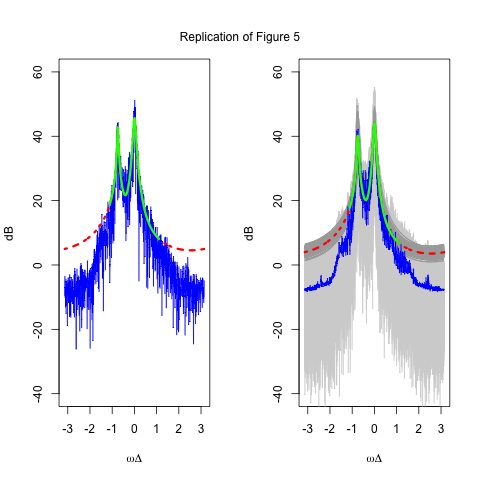
\includegraphics[width=.5\textwidth]{fig5.png}
        \caption{Left: The spectral density of one particle (blue) with the model fit overlaid for the portion of the spectra used to fit it (green) and extended to all frequencies (red). Right: The ensemble mean periodogram (blue) with the ensemble fit for the frequencies used to fit it (green) and extended to the entire spectrum (red) and individual trajectories' periodograms (light grey) and model fits (dark fit) }
\end{figure}

We also consider the trajectory of a drifter in the South Pacific Ocean observed 12 times a day over a 1642 day period. Using a rolling window of 1000 observations and the semi-parameteric set-up described in Section X, we obtain parameter estimates for the spectral model at each time point. In Figure ~\ref{fig:timeVarying}, we compare the observed spectral density over time and the fitted spectral density. The fitted density appears to be a smoothed version of the observed density, indicating a reasonable model fit. We also display the fitted parameter values over time and their 95$\%$ confidence interval bands in Figure 8 (add fig and renumber) and report the correlation among variables in Figure 10 (and fig and renumber). 

We also fit a 5-parameter where the frequency is set to the inertial frequency rather than being a free-parameter. We then compare the fit to the full model using a likelihood ratio test as described in Section X. In Figure 9, we display the test statistic over time where a red line is used to indicate the level of statistical significance. We conclude for time periods where the test statistic is greater than this cut-off that there is a shift in the inertial frequency. 


\begin{figure}[hb]
	\label{fig:timeVarying}
  \centering
    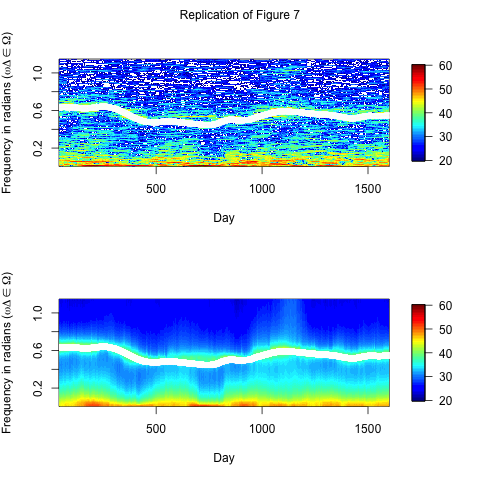
\includegraphics[width=.5\textwidth]{fig7.png}
        \caption{Top: Observed spectra of the drifter over time; Bottom: Modeled spectra over time. On both figures, the white line indicates the average inertial frequency within the rolling window at the current time period.  Only frequencies used in the estimation are included.  }
\end{figure}

\section{Discussion}
identifiability 



\clearpage

\bibliography{prelim}


\section{Appendix}

\subsection{Errata}

\subsection{Additional Figures}


\end{document}

